\chapter{Implementation}
\label{chap:implementation}

The development of the project was carried out in several iterations, while each 
improving upon the last in terms of functionality and modularity.
The first two iterations were carried out using the Poke-env library, and a 
custom agent. The last iteration focused on the implementation of a custom 
environment and changeing the agent to use the custom environment.


We can refer to Chapter~\ref{chap:analysis-and-design} for something.

\section{Iteration 1: Agent and a Pokemon environment} 
\label{sec:Iteration-1-Agent-Environment}

The first iteration of the implementation focuses on having a minimum viable product \(MVP\). The MVP
consists of all MUST (M) requirements, which can be used as a baseline for next iterations.
Look chapter \ref{sec:functional-requirements} for a complete list of the MUST have requiremetns.
The MVP consists of a custom agent, with a custom training loop, that plays against a poke-env random agent,
in a generation 9, single battle pokemon showdown environment, where held items are available. 

\subsection{Poke-env Library}
The backbone of the first iteration of implementation is the Poke-env library. 
To simulate pokemon battles, we wrap our agent in a custom player class which inherits from the
Poke-env player class. This allowed us to model battles in any pokemon showdown 
provided battle format, such as Single or Double battles and retrieve relevant game information.
The agent was embedded into the environment, and could interacted through asynchronouns function
to reflect the turn-based format of pokemon battles.


\subsection{Deep Q-Network Agent}
The agent is implemented using a Deep Q-Network (DQN) model. This approach leverages
a nerual network to approximate the Q-values, enabling the agent to learn an 
effective policy directly from the environments state representation. 
The Q-network was constructed using Pytorch and consists of a simple feedforward
architecture with two hidden layers. 
\begin{lstlisting}[basicstyle=\fontsize{10}{10}\selectfont\ttfamily,language=Python,caption={The defined action space.},label=lst:action-space-def,breaklines]
class DQN(nn.Module):
    def __init__(self, state_size, action_size):
        super(DQN, self).__init__()
        self.fc1 = (nn.Linear(state_size, 64)) #Input layer -> Hidden layer
        self.fc2 = (nn.Linear(64, 64)) #Hidden layer -> Hidden layer
        self.fc3 = (nn.Linear(64, action_size)) #Hidden layer -> Output layer

    def forward(self, x):
        x = torch.relu(self.fc1(x))
        x = torch.relu(self.fc2(x))
        x = self.fc3(x)
        return x 
\end{lstlisting}
This structure includes:
\begin{itemize}
    \item An input layer, that processes the state representation.
    \item Two hidden layers, each with 64 neurons and ReLu (rectified linear unit function) activations.
    \item An output layer, that produces Q-values for each possible action.
\end{itemize}

\subsubsection{State Representation and Action Space}
The state representation is a simple embedding consisting of the normalized Hit Point (HP) values
for the active pokemon and opponent. The action space is a flattend list that
include all available actions in the current state, such as moves, switching pokemon
or using items. These 2 features are simplified yet informative and generalized 
enough to be used in the two core formats of the pokemon game.

\subsubsection{Exploration, Learning Process and Training configuration}
To manage the exploration-exploitation trade-off, an epsilon-greedy ploicy is employed.
The epsilon value stats at 1.0, allowing the agent to explore in the early stages of training,
where after it decays after each episode with a factor of 0.995 with a lower bound of 0.05.
This ensures that the agent gradually shifts from exploration early in training
and focuses more on exploitation later on.
A replay buffer is used to store the agent's transitions (state, action, reward, next-state, done), 
and are sampled in batches for training, which can help stabilize the learning process 
by reducing correlations between sequential experiences. Furthermore, a target 
network is periodically updated to improve learning stability.
The agents was trained using the following hyperparameters:
\begin{itemize}
    \item \textbf{Batch Size:} 64
    \item \textbf{Replay Buffer Size:} 100000
    \item \textbf{Learning Rate:} 0.001 
    \item \textbf{Epsilon:} 1.0
    \item \textbf{Epsilon Decay:} 0.995
    \item \textbf{Epsilon Min:} 0.05
    \item \textbf{Tau:} 0.005
    \item \textbf{Gamma:} 0.99
\end{itemize}

\subsubsection{Limitations and Challenges}
while the first iteration of the implementation was successful in creating a custom agent
and training loop, it was faced with soem limitations and challenges.
\begin{itemize}
    \item The training loop was constrained to only single battle formats, with
    randomly generated teams, for both agents, for each episode. This was done to create a
    more generalzed agent, but introduced a high variance in the training process and came with more challenges.
    \item In some cases, the agent would be unable to finnish the training process, due to the 
    opponent agent not able to finish the battle. It would get stuck in a loop, trying to switch when it
    wasnt a valid action.
\end{itemize}
\section{Iteration 2: Agent Improvements}
\label{sec:Iteration-2-Agent-Environment}
The second iteration of implementation focused on restructuring the agent for improved 
modularity, better representation of game states and scaleability. This version of the agent still
uses the Poke-env library, but the agent is now training in a double battle environment. The
agent is now capable of handling multiple Pokemon and can make decisions based on the state of 
both opponent pokemon and allied pokemon. The agent also uses PyTorches own replay buffer for
training, which is a significant improvement over the previous custom version.

\subsection{Agent}
Our agent is now capable of accepting pre-made teams so long a team alligns with the required battle
format. The agents hyperparameters are now also much more modular, allowing for easy tuning and
we have moved the training loop inside the agent class, so that the asynchronous methods only
sends and accept challenges from the agent in the environment. The state size is now also 
calculated based on the number of pokemon in the team, and the number of pokemon in the opponents 
and their type. This means we have a lot more options for the agent to choose from, and learn 
the pokemons types. This also means that the Q-function approximator is now a lot more complex,
because the agent is now capable of learning from a much larger state space. 


\subsection{Reward Function}
This new reward function is an improvement over the previous one, as it now takes into accounts
the HP of the all pokemon on the field, and the amount left after the battle. The reward function
is an important part of the training process, as it not only gives us visual data to measure, but
also allows the agent to learn and adapt to the environment. This will give us a better understanding
of how well the agent is learning and its performance. In the previous iteration, the reward
function only gave a reward based on winning and losing, and taking an average of og the number of
times won and lost gave us a flat curve, because there was no real variation in the data.
The new reward function could also be further improved, by adding a reward for a number of turns
or increasing the reward for a winning streak. This would allow the agent to make a repoducable output
quicker, and would also allow us to measure the agents performance over time.
The reward function is as follows:


\subsection{Replay Buffer} % Explain 
There are two parts to the replay buffer, the first is storing observed experience tuples in a replay 
memory, and the second is to push small batches of experience tuples randomly, to help train the agent. 
The replay buffer is a key part of the training process, as it allows the agent to learn from its own 
experience, and allows us to update our target Q-network dynamically during training. The experience
tuples stored are as follows: 
\begin{itemize}
    \item \textbf{State}
    \item \textbf{Action}
    \item \textbf{Reward}
    \item \textbf{Next State}
    \item \textbf{Done}
\end{itemize}






% We refer to Listing~\ref{lst:sum} for the Java implementation.\\ % force new line
% Code snippets like \lstinline{System.out.println} can also be given inside a sentence.

% \begin{lstlisting}[language=java,caption={Our sum implementation},float=tb,label=lst:sum]
%   class Sum {
%     public static void main(String[] args) {
%       int n = 5;   // the input
%       int sum = n * (n+1);
%       System.out.println("The sum is: " + sum);
%     }
%   }
% \end{lstlisting}

% Finally we can refer to some material in Appendix~\ref{appendix:api-doc}. 

\section{Environment}
\label{sec:environment}

\subsection{Structure}
OOP
Modules
Separation of concerns

\subsection{Team builder}

\subsection{Team parser}

\subsection{Gymnasium environment}
Action spaces
Observation spaces
Stepping

\subsection{Pokemon domain}
The custom environment is modelled from a real Pokemon battle environment from the 9th generation of Pokemon as described in the project requirements.
This environment was broken down into 4 parts:
\begin{itemize}
    \item Pokemon
    \item Battlefield
    \item Turn processing
    \item Move handling
\end{itemize}

\subsubsection{Pokemon}
First a Pokemon had to be modelled in order to be used in the environment.
To get the Pokemon's data a separate module was created. A pokemon-team-builder-cli \cite{TeambuilderCli} tool that
fetched data from Pokeapi \cite{PokeAPI} and marshalled the responses into a shape that was useable by our domain.
In order to save the created teams and share them between users of the project, they were saved as JSON objects.
The teams are then able to be loaded via the project's data module that parses the JSON back into valid Pokemon.
The Pokemon are modelled as Python dataclasses that maintain all the information related to a specific Pokemon, such as
its stats, moves and current boosts and status conditions. When the Pokemon is first initialized, its actual stats
are calculated from the species base stats and the its IVs and EVs (see listing \ref{lst:stat-calc}). This allows the teambuilder to be
completely unaware of the actual implementation of the data it provides and allows us to adjust how stats are handled
without having to remake the initial data.

\begin{figure}[h]
    \centering
    \begin{lstlisting}[basicstyle=\fontsize{10}{10}\selectfont\ttfamily,language=Python,caption={Function for calculating a Pokemon's stats.},label=lst:stat-calc,breaklines]
    def _calculate_stat_value(self, stat: PokemonStatKey) -> int:
        nature_modifier: float = self.get_nature_modifier(stat)
        stat_value = self._base_stats.get(stat)
        iv_value = self._ivs.get(stat)
        ev_value = self._evs.get(stat)
    
        [...]
    
        if stat == 'hp':
            return math.floor(((2 * stat_value + iv_value + ev_value // 4) * self.level // 100) + self.level + 10)
            
        return math.floor((((2 * stat_value + iv_value + ev_value // 4) * self.level // 100) + 5) * nature_modifier)
    \end{lstlisting}
\end{figure}

\subsubsection{Battlefield}
The next step in setting up the environment is creating the battlefield that the Pokemon are using. In order to keep track
of all the actions that are taken a \lstinline|BattleState| class is created. The \lstinline|BattleState| keeps track of
each turn that has happened in a battle and logs every action taken to be easily reviewed later in case something goes wrong,
or the user wants to see an example of the AIs behavior (see listing \ref{lst:sample-log}).
\begin{figure}[H]
    \centering
    \begin{lstlisting}[caption={Sample log from an episode.},label=lst:sample-log,breaklines]
        Turn 1:
        - toxapex used protect on toxapex
        - shiftry used grassy-glide on toxapex
        - toxapex protected itself
        Turn 2:
        - shiftry used sucker-punch on toxapex
        - it's not very effective
        - toxapex took 39 damage
        - toxapex used poison-jab on shiftry
        - it's super effective
        - shiftry took 126 damage
    \end{lstlisting}
\end{figure}

The \lstinline|BattleState| keeps track of each players team as well as their active Pokemon. Only the active Pokemon are able to
perform actions on a given turn. The active Pokemon are stored in a \lstinline|List| which is then used to help determine
the correct turn order.

Finally, the \lstinline|BattleState| holds the \lstinline|BattleEffectsManager|. This class maintains all the field wide
effects in a battle such as weather, terrain and barriers. It handles adding the various effects to the battle, processes
their effects and ensures that they fade away when they are meant to.

\subsubsection{Turn processing}
A Pokemon battle is composed of actions taken every turn. There are many effects that take place at various stages of a turn.
For instance, most status conditions have their turn counter decremented at the beginning of a turn and have their effects trigger at
the end of a turn. The \lstinline|step()| function defines the turn order of operations as start of turn, actions and end
of turn (See figure \ref{fig:turn-order-of-operations}).

\begin{figure}[H]
    \centering
    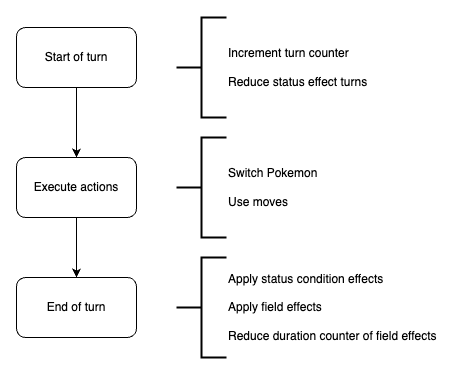
\includegraphics[width=.75\textwidth]{assets/turn-order-of-operations.png}
    \caption{Turn order of operations.}
    \label{fig:turn-order-of-operations}
\end{figure}

Entities with start of turn or end of turn effects expose a \lstinline|on_turn_start| or \lstinline|on_turn_end| function
that can be called inside the step function (see listing \ref{lst:turn-end-func}). This is based on
the Facade design pattern and makes sure the environment doesn't need to know the full details of how each entity needs
to be handled. This approach is also partially inspired by an observer pattern as the relevant entities are "subscribed"
to the start/end of turn events in the environment.
\begin{lstlisting}[language=Python,caption={Example of the environment handling the end of a turn without knowing each entity's full implementation.},float=h,label=lst:turn-end-func,breaklines]
def on_turn_end(self, sorted_active_pokemon: list[Pokemon]):
    for pkm in sorted_active_pokemon:
        pkm.on_turn_end()
    self.state.battle_effects_manager.on_turn_end(sorted_active_pokemon)
\end{lstlisting}

\subsubsection{Move handling}
There are many categories of moves in Pokemon that have to be handled in different ways. In the teambuilder \cite{TeambuilderCli},
move data is gathered together with the Pokemon. We use the data to determine which category a move belongs to and thus how
to handle it. Move handling is defined in the \lstinline|BattleActions| class. If the agent chooses a move as its action
the \lstinline|BattleActions.executeMove| method is called (see listing \ref{lst:exec-move-func}). This method checks the 
move's category and matches it to the appropriate handler to calculate how much damage is dealt, how much health is restored 
and whether or not a secondary effect occurs.

\begin{lstlisting}[basicstyle=\fontsize{10}{10}\selectfont\ttfamily,language=Python,caption={Excerpt of the execute move function.},float=h,label=lst:exec-move-func,breaklines]
def execute_move(self, move: PokemonMove, attacker: Pokemon, target: Pokemon):
    if not self._can_execute_move(attacker, move, target):
        return

    inflicted_damage = 0
    restored_health = 0

    match move.category:
        case 'ailment':
            self._handle_ailment_move(move, target)
        case 'damage':
            inflicted_damage = self._handle_damage_move(move, attacker, target)
        case 'damage+ailment':
            inflicted_damage = self._handle_damage_with_ailment_move(move, attacker, target)
        [...]
        case 'damage+lower' | 'damage+raise':
            inflicted_damage = self._handle_damage_with_stat_change(move, attacker, target)
        case 'damage+heal':
            inflicted_damage = self._handle_damage_with_healing(move, attacker, target)
            restored_health = math.floor(inflicted_damage * (move.drain / 100))
        [...]
        case 'field-effect':
            self._handle_field_effect(move, target)
        case 'unique':
            self._handle_unique_move(move, target)

    self._apply_move_effects(move, attacker, target, inflicted_damage, restored_health)
\end{lstlisting}

Damage is calculated using a close approximation of the official Pokemon damage formula, however due to not implementing 
the full set of Pokemon mechanics it is not entirely faithful and will deviate from reality by a small amount. When comparing
to a fully featured damage calculator the implementation is usually off by 1 or 2 damage points. This may also be caused 
by the alternative rounding rules utilized by the Pokemon games, as the official games round down at 0.5 and it is not well-documented
where exactly rounding occurs in the formula. However, as this deviation is the same for both agents it was deemed to be 
good enough in terms of creating a faithful simulator.

